\documentclass[12pt]{article}
\setlength{\parskip}{\baselineskip}
\usepackage{fullpage}
\usepackage{graphicx}
\usepackage{underscore}
\usepackage{amsmath,amsfonts,amssymb}

\title{Homework 2}
\author{CSCI 4511W Spring 2018}
\begin{document}
\date{February 15, 2018}
\maketitle

Instructor: Dr.Maria Gini\hfill Joowon Kim(kimx4342)

\hrulefill

\begin{enumerate}
\item You are given the following heuristic function for the Traveling SalesPerson Problem (TSP): h(n) = distance to the closest unvisited city. Answer the following questions:
  \begin{enumerate}
  \item Is this heuristic admissible? Explain your reasoning. \par
  
  Yes, this is heuristic admissible. The condition of admissible is that we shouldn't overestimate the cost to the goal state, It's because there must visit all of the node so that the distance to the closest city that is not visited yet can never be greater distance to it.
  
  \item Show an example of a TSP where Greedy-Best-First algorithm with this heuristic finds an optimal solution \par
  
  Let's say there are 5 cities and set the starting city as a city 1. The distance between city1 and city2 is $1$, city1 and city3 is $2$, city1 and city4 is $3$, city1 and city5 is $4$, city2 and city3 is $10$, city2 and city4 is $8$, city2 and city5 is $3$, city3 and city4 is $9$, city3 and city5 is $7$, city4 and city5 is $5$. It will go city2, than city5. After that, it will chose city4 than city3 and back to city1 after visiting all of the cities. The cost is $1+3+5+9+2=20$ which is the least cost and it is an optimal solution. 
  
  \item Show an example of a TSP where the Greedy-Best-First algorithm with this heuristic does NOT find an optimal solution \par
  
   Let's say there are 5 cities and set the starting city as a city 1. The distance between city1 and city2 is $1$, city1 and city3 is $2$, city1 and city4 is $3$, city1 and city5 is $4$, city2 and city3 is $10$, city2 and city4 is $8$, city2 and city5 is $3$, city3 and city4 is $9$, city3 and city5 is $7$, city4 and city4 is $5$. From the starting city, which is city1, it goes to city5, city4, city3, city2 and city1. It visited all of the cities and the cost is $4+5+9+10+1 = 29$, and this is not an optimal solution. 
  
  \item Is Greedy-Best-First search with an admissible heuristic guaranteed to find an optimal solution? \par
  
  With the Greedy-Best-First search, we cannot guarantee to find an optimal solution. It only see the cost to the next node and cannot see the distance it traveled. Also,  when the total path cost is greater than the alternative one, it cannot track.
  
  \item Propose an admissible heuristic for the TSP, different from the heuristics given above. \par
  
  $h(n)$ = shortest distance to the cities from the start
  
  \end{enumerate}

\item What are the disadvantages of using a heuristic function for A* which is NOT consistent? \par

	If the heuristic is admissible and not consistent, the node may be moved back from the closed list to the open list. Also, there will be risk of more node expansions. A* will re-expand the node if not consistent heuristic is used. 

\item The terms g and h each play a different role in A*. What are those roles? What happens when you emphasize or de-emphasize one of them by using different weights in f(n)? Consider the case in which f(n) = (1-w)g(n) + wh(n), with 0 <= w <= 1. Be specific and analyze what happens for different values of w. \par

	\(f(s) = g(s) + h(s)\). \par
    \(g(s)\) is the cost from starting point to the state s and \(h(s)\) is the heuristic estimated cost from state s to goal. If \(g(s)\) is more emphasized, the heuristic value would be trivial so A* will degrade into Uniform Cost search. Otherwise, if \(h(s)\) is more accentuated, A* will act like Greedy-Best-First-Search by expanding the most promising node according to its heuristic function.

\item Why any heuristic which is an optimal solution to a relaxed problem is admissible and consistent? \par

	To get an optimal solution, it needs admissible and consistent heuristic. The heuristic does not overestimate the cost. If it does, it might overlook the optimal path and yield to the wrong solution. And if not consistent, there can be other path that is less cost than the current one. So it also has to be consistent.

\item In A* the nodes that have been generated but not yet expanded are sorted according to the value of f(n) = g(n) + h(n), i.e. the sum of the cost from the start to node n plus the estimated cost from n to goal using admissible heuristic h(.). Nodes that have the same f(.) value are ordered arbitrarily. 
Propose a domain independent criterion that could be used to order the nodes with the same f(.) value. Explain your answer. \par
	
    If the same f(.) value is arranged by g(.) value, it can be a domain independent criterion. Assume there are two nodes that have an f(.) value that has a total cost of 100 by adding g(.) value of 90 and h(.) value of 10. It shows that majority of f(.) value is a real cost rather than an estimated cost and indicates that the goal is almost reached. In contrast, if the f(.) value is consisted of g(.) value of 10 and h(.) value of 90, it implies that the most of the cost is estimated and possibly underestimated. So the costs stand a good chance of going up.  
    
\item Discuss the possible advantages of the following state-space search strategy: obtain by some method a path to a goal node and its associated cost f(Goal)=C. This cost is not necessarily minimal but it gives an upper bound on the minimal cost. Now use A* with an admissible $h$ function and discard immediately any OPEN nodes reached whose f values are greater than C.
  \begin{enumerate}
  \item Explain if the modified A* algorithm with this strategy is guaranteed to find an optimal solution if one exists or not. Be short but precise. \par
  
  It is not guaranteed to find an optimal solution. The C value is not exact minimal cost so that we cannot say we can always find an optimal solution.
  
  \item Explain if the fact that the algorithm discards some of the OPEN nodes (i.e. nodes in the frontier) means that fewer nodes are expanded. Be short but precise. \par
  
  The algorithm discards some of the OPEN nodes does not mean that fewer nodes are expanded. Since there are some other nodes that has the lower f values, OPEN nodes whose f values are greater than C can be less expanded. Eventually, the number of nodes that are expanded doesn't really affect the result. 
  
  \item Does this strategy reduce the total storage requirements? Explain your reasoning. \par
  
  This strategy reduce the total storage requirements. In original, they keep all open node but with this strategy that discards some of the OPEN nodes can save the memory. So the algorithm using this strategy has less storage requirements compare to the original algorithm. 
  
  \end{enumerate}

\end{enumerate}

\newpage

PROGRAMMING QUESTIONS
\begin{enumerate}
\item 
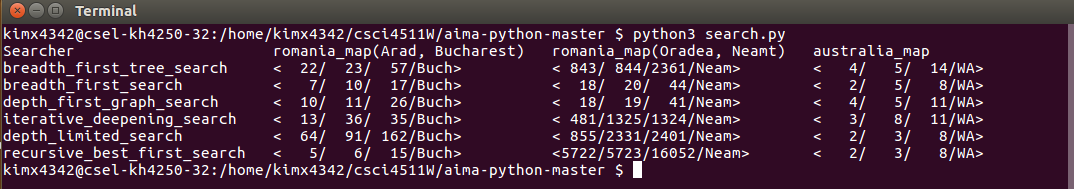
\includegraphics[width=\textwidth]{prob1.png} \par
\item
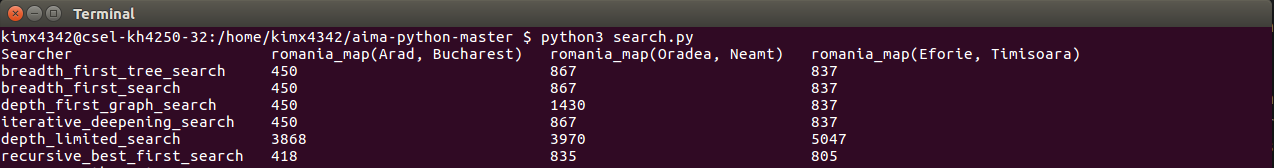
\includegraphics[width=\textwidth]{prob2.png} \par
\item
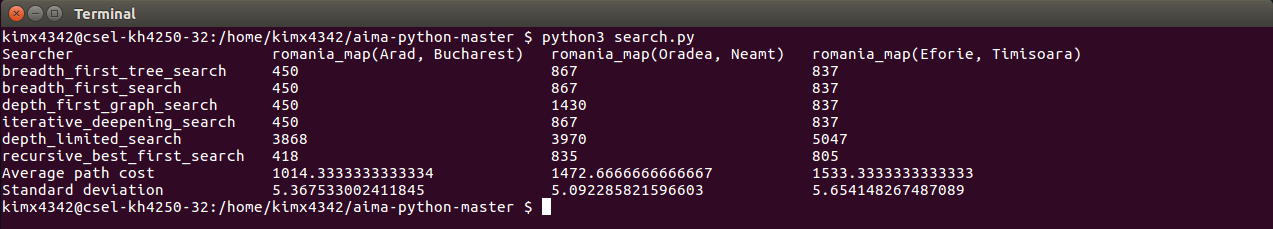
\includegraphics[width=\textwidth]{prob3.png} \par
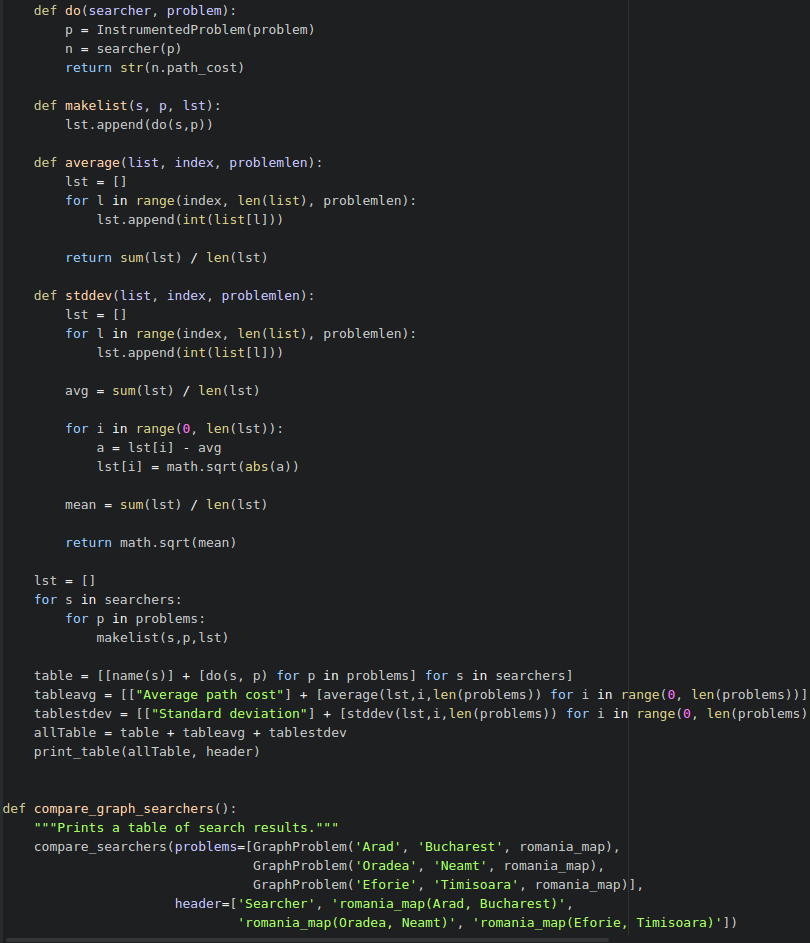
\includegraphics[width=\textwidth]{code.png}
\end{enumerate}

\end{document}